% Use the elsarticle class and bibliography style supplied with this template.
\documentclass[preprint,12pt]{elsarticle}

\usepackage{amssymb}
\usepackage{amsmath}
\usepackage{graphicx}
\usepackage{subcaption}
\usepackage[colorlinks]{hyperref}
\hypersetup{
  citecolor=blue,
  linkcolor=blue,
  urlcolor=blue,
  pdftitle={AI-assisted data discovery and analysis for solar physics: the StiXpert approach},
  pdfauthor={Hualin Xiao}
}
\usepackage[utf8]{inputenc}
\usepackage[capitalise,noabbrev]{cleveref}

\journal{Astronomy and Computing}

\begin{document}

\begin{frontmatter}

  \title{StiXpert: AI-assisted knowledge discovery and data analysis
    for solar physics}

  \author[inst1,inst2]{Hualin Xiao\corref{cor1}}
  \ead{hualin.xiao@fhnw.ch}
  \cortext[cor1]{Corresponding author}

  \address[inst1]{University of Applied Sciences and Arts Northwestern
    Switzerland (FHNW), Switzerland}
  \address[inst2]{Physikalisch-Meteorologisches Observatorium Davos/World
    Radiation Center (PMOD/WRC), Davos, Switzerland}

  \begin{abstract}
    Solar-flare studies combine observations and analysis software from multiple
    instruments.
    We present StiXpert, an AI-assisted service developed around STIX for retrieving
    solar-physics knowledge, discovering relevant observations and methods, and
    supporting analysis code.
    Its knowledge base includes solar-physics context, STIX instrument knowledge and
    software, STIX Data Center resources, and selected SSWIDL material spanning multiple
    instruments.
    Its main capabilities are knowledge discovery and assistance with data analysis,
    supporting solar research across instruments.
  \end{abstract}

  \begin{keyword}
    Solar physics \sep Solar flares \sep STIX \sep Artificial intelligence
    \sep Knowledge base \sep Data discovery \sep Scientific software
  \end{keyword}

\end{frontmatter}

\section{Introduction}
\label{sec:intro}

Solar-physics research often combines observations from instruments that differ in energy
range, cadence, observing mode,  and data products.
A flare study may bring together hard and soft X-rays, solar energetic
particles, extreme-ultraviolet images, radio measurements, and observations from
spacecraft at different locations.
Researchers must identify which observations cover an event, select suitable products,
and understand the assumptions behind their analysis.

The software used to carry out this work is similarly distributed.
SolarSoft/SSWIDL provides a long-standing environment for solar-data analysis
\cite{freeland1998}; the Python ecosystem includes SunPy for solar research
\cite{sunpy2020} and Astropy for general astronomical tasks such as time, coordinates,
and units \cite{astropy2018}.
Instrument teams also maintain dedicated software for accessing, calibrating, and
analyzing their data, using IDL, Python, or other environments.
Moving among these resources can make it difficult to find the appropriate routine,
product, or method, particularly in studies that combine several instruments.

Large language models (LLMs) can answer general questions and assist with code writing,
but their broad capabilities do not ensure detailed knowledge of solar phenomena,
instrument capabilities, let alone the data products, analysis methods, the software used to apply
them.
Retrieval-augmented generation (RAG) can ground answers in relevant source material
\cite{lewis2020}, while tool-mediated agents can retrieve and use that information in
successive steps \cite{yao2023}.
Providing AI with this domain-specific knowledge can support scientific knowledge
retrieval, observation and method discovery, as well as code development and analysis
workflows when these are needed.

Here we present StiXpert, an AI service developed around the Spectrometer/Telescope for
Imaging X-rays (STIX), a hard X-ray imaging spectrometer onboard Solar Orbiter that
provides spectral and imaging diagnostics of solar flares \cite{krucker2020}.
StiXpert makes indexed instrument knowledge, data-product information, analysis
software, and related scientific context available to AI clients through retrieval
and tool-based interactions.
Although STIX is the organizing use case, the indexed knowledge also includes selected
SolarSoft/IDL resources covering multiple instruments and broader solar-physics
context.
StiXpert is therefore intended to support knowledge discovery as well as code
assistance. As we also ingested broader solar-physics knowledge and \texttt{SSWIDL} source code, 
 the system can support research beyond STIX.
\section{StiXpert: architecture and interaction model}
\label{sec:architecture}

\subsection{Design objectives}

The system addresses three connected tasks: retrieving relevant scientific knowledge;
using it to identify candidate observations, data products, and analysis methods; and,
when needed, helping the researcher express a selected workflow in the language and
environment they use.
The implementation is anchored in STIX data and expertise, while its indexed SSWIDL
routines, complementary Python packages, and solar-flare and Solar Orbiter context
support workflows that combine STIX with observations from other instruments.
STIX is the organizing use case, not a boundary on the scientific questions and
software that the knowledge base can support.

The design follows four principles.
First, answers to scientific and instrument-related questions should be grounded in
indexed material rather than depend only on model memory.
Second, the assistant should help researchers discover relevant observations, data
products, methods, and supporting software.
Third, any resulting analysis code should be inspectable and run in the researcher's own
environment.
Fourth, the assistant should communicate uncertainty and leave scientific
interpretation and acceptance of results to the researcher.

\subsection{Knowledge and service layers}

\Cref{fig:architecture} summarizes the architecture.
The index builder statically parses selected source trees and stores searchable records
in a SQLite knowledge base; indexed code is not imported or executed during indexing.
Python sources include stixpy, stixdcpy, sunkit-spex, and solo-epd-loader, with
selected examples and documentation.
The index also includes SSW/IDL routines and supporting configuration and text data,
selected STIX Data Center browser scripts, and descriptions of public data-centre
routes and their parameters, as well as indexed context on solar flares and Solar
Orbiter.
The route index excludes endpoints classified as private or mutating.
This is a software- and source-grounded resource: the indexed SSW material spans
multiple solar instruments, whereas the Python sources and data-centre descriptions
provide stronger STIX-specific coverage.
The combination supports questions that connect STIX with complementary observations
without implying uniform documentation coverage for every instrument.

An MCP server presents retrieval tools and workflow guidance to a compatible AI client.
This gives the model a structured means to search and inspect relevant material rather
than answer solely from its pretrained memory.
In a RAG interaction, a question about a flare can lead first to retrieved information
on its scientific context, instrument coverage, available products, and relevant
methods.
The researcher may then use that information to refine the scientific question or
choose whether to proceed to an analysis workflow and code.
Such retrieval can be useful in its own right; a program need not be generated for the
assistant to help clarify what is known or which observations may address a question.
Retrieved material supports an answer but does not, by itself, establish that a proposed
method is appropriate or that a generated program is correct.

\begin{figure}[htbp]
  \centering
  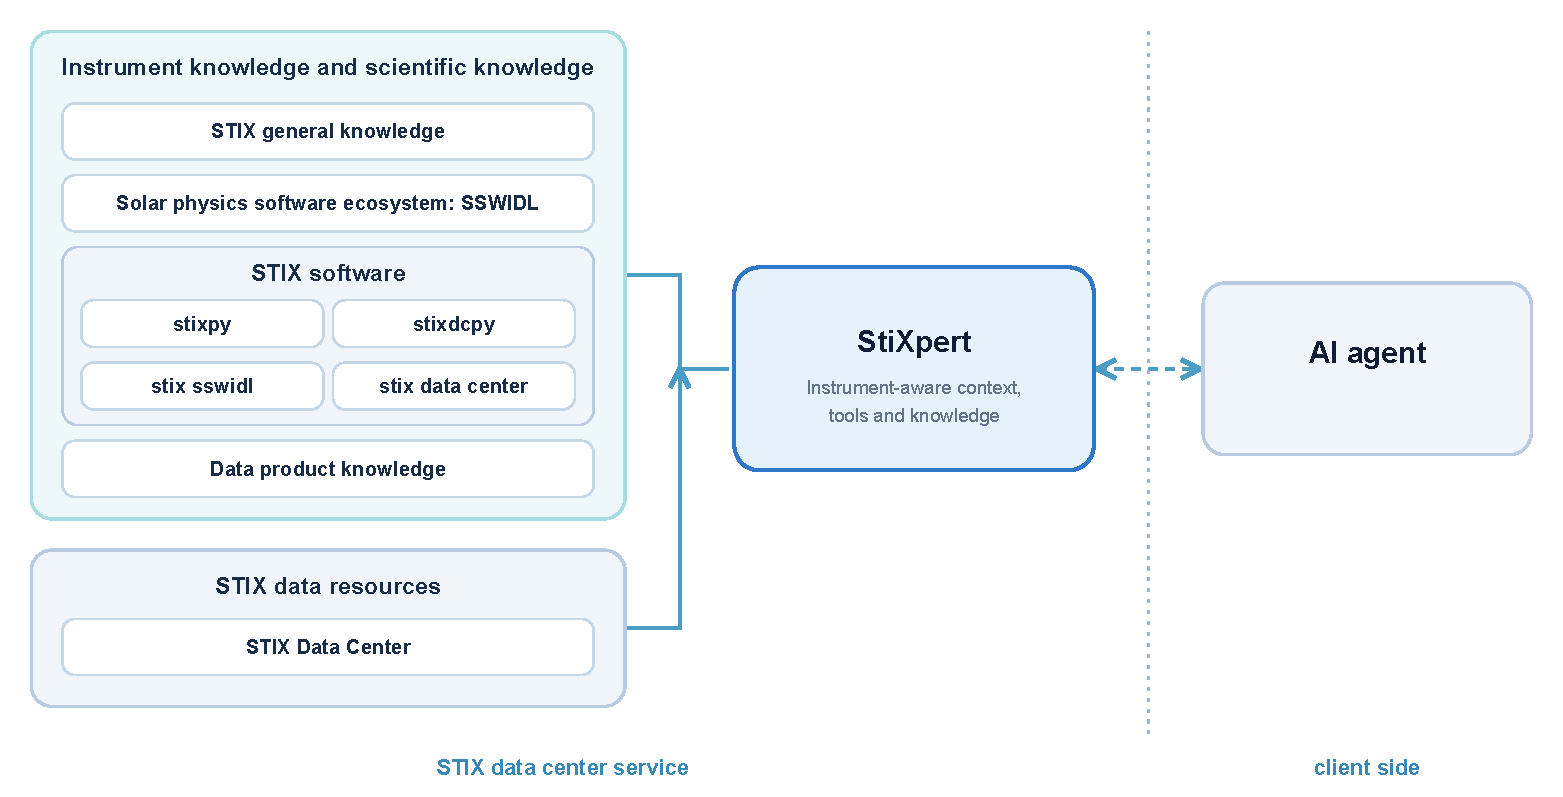
\includegraphics[width=\linewidth]{figures/stixpert-architecture.pdf}
  \caption{StiXpert architecture.
    STIX knowledge and data-centre resources are combined with broader solar-physics
    context and software, including SSWIDL routines relevant to multiple instruments.
    These indexed resources are made available to an MCP-compatible AI client for
    knowledge retrieval and scientific discovery, with code assistance as a possible
    subsequent step.
    The diagram depicts the knowledge and service boundary; it does not imply autonomous
    scientific validation or execution by the knowledge-base server.
  }
  \label{fig:architecture}
\end{figure}

\subsection{From a scientific question to retrieval and analysis}
\label{sec:workflow}

The assistant first interprets the user's prompt to identify the scientific question
and the information or analysis requested.
For a knowledge question, it searches the indexed material and returns relevant
scientific context, publications, instrument descriptions, data-product information,
methods, or software guidance.
This retrieval can answer a question directly; code generation is not required.

When the user requests an analysis, the assistant uses keyword and semantic search to
find the resources most relevant to the prompt.
It first seeks an applicable, predefined workflow.
For example, a STIX flare workflow may identify events, retrieve quicklook and pixel
data, perform spectral analysis with \texttt{sunkit-spex}, and reconstruct images with
\texttt{stixpy}.
For IDL, it searches for corresponding SSWIDL procedures and configuration guidance;
the Python and IDL workflows are related but are not assumed to be identical.
If no predefined workflow is suitable, the assistant searches indexed examples and
source code for relevant procedures or functions, then uses those findings to formulate
an analysis sequence and draft code.

Before code is provided, the assistant can check candidate workflows and routines
against retrieved documentation and examples.
For Python, the reference service also supports static syntax and selected-reference
validation.
These checks do not execute an analysis or establish that its scientific results are
correct: runtime testing with appropriate data must be performed in the user's
environment.
The MCP service itself searches its local index and does not fetch STIX data or run
analysis scripts.
In the example described below, the generated IDL procedure could not be run and
therefore remains unverified.

StiXpert can also assist with translating code between Python and IDL, including adapting
an existing routine when no direct counterpart is indexed.
Such translation is a proposed implementation, not evidence of equivalent behavior;
the researcher must check the translated method, inputs, assumptions, and outputs.

\section{Illustrative assistant interactions}
\label{sec:demonstrations}

The following examples illustrate code assistance in two analysis environments: a
Python notebook that explores a recent STIX flare list and its quicklook light curves,
and an IDL program draft for a STIX--GOES light-curve comparison.
These examples do not evaluate the accuracy or completeness of RAG-based
knowledge-retrieval answers.
They are illustrative demonstrations, not a controlled benchmark.
The examples concern light curves only; they do not establish performance in spectral
fitting, image reconstruction, source translation, or physical interpretation.

\subsection{Python notebook: STIX event and light-curve exploration}
\label{sec:python-demo}

The Python interaction began with a request to create a Jupyter notebook that queries
recent solar flares and displays their light curves.
Scientifically, this provides an exploratory view of which events and quicklook
measurements were returned for the requested interval, before the user selects an event
for closer study.
The assistant produced a notebook that, according to the accompanying explanation,
queried the STIX flare list and five-band quicklook light curves through
\texttt{stixdcpy}, converted the returned count arrays to a time-indexed table, shaded
flare intervals, plotted an overview on a logarithmic count scale, and created a set of
closer views around selected events.
The visible plot labels the five energy bands as 4--10, 10--15, 15--25, 25--50, and
50--84~keV, with a nominal four-second count bin.

The notebook output reports 58\,580 time samples, from 2026-11-16 09:23:28 to
2026-11-19 02:28:44~UTC.
The assistant's summary reports 193 flares in the requested three-day window and
identifies an M1.7 event on 2026-11-17 at 21:38~UTC as the strongest in that returned
list.
The assistant also notes that the final light-curve sample precedes the requested
window end by approximately seven hours.
This discrepancy is visible in the example and was not independently attributed to
data-centre latency; the plot should therefore be treated as an exploratory quicklook
rather than a completeness-checked event product.

\subsection{IDL draft: STIX and GOES light curves}
\label{sec:idl-demo}

The second request asked for an IDL program to plot STIX light curves for 2026-02-01 to
2026-02-02 together with GOES X-ray flux.
The generated procedure draft uses the STIX quicklook light-curve routines for five
energy bands and requests one-minute GOES-18 and GOES-19 flux in two wavelength
channels.
This example demonstrates that an assistant can draft code that combines
instrument-specific SSWIDL routines with data from another observatory.

The IDL environment was not installed or configured in the session shown in
\Cref{fig:assistant-code-examples}; the assistant explicitly reports that the procedure
could not be run and remains unverified.
Accordingly, the figure documents code generation only.
It does not show a successful IDL execution, a comparison with the Python output, or
scientific equivalence of the two analyses.
Verification would require running the code in a configured SSWIDL environment and
inspecting the returned GOES structure, time conversion, plot axes, and data coverage.

\begin{figure}[htbp]
  \centering
  \begin{subfigure}[t]{0.49\linewidth}
    \centering
    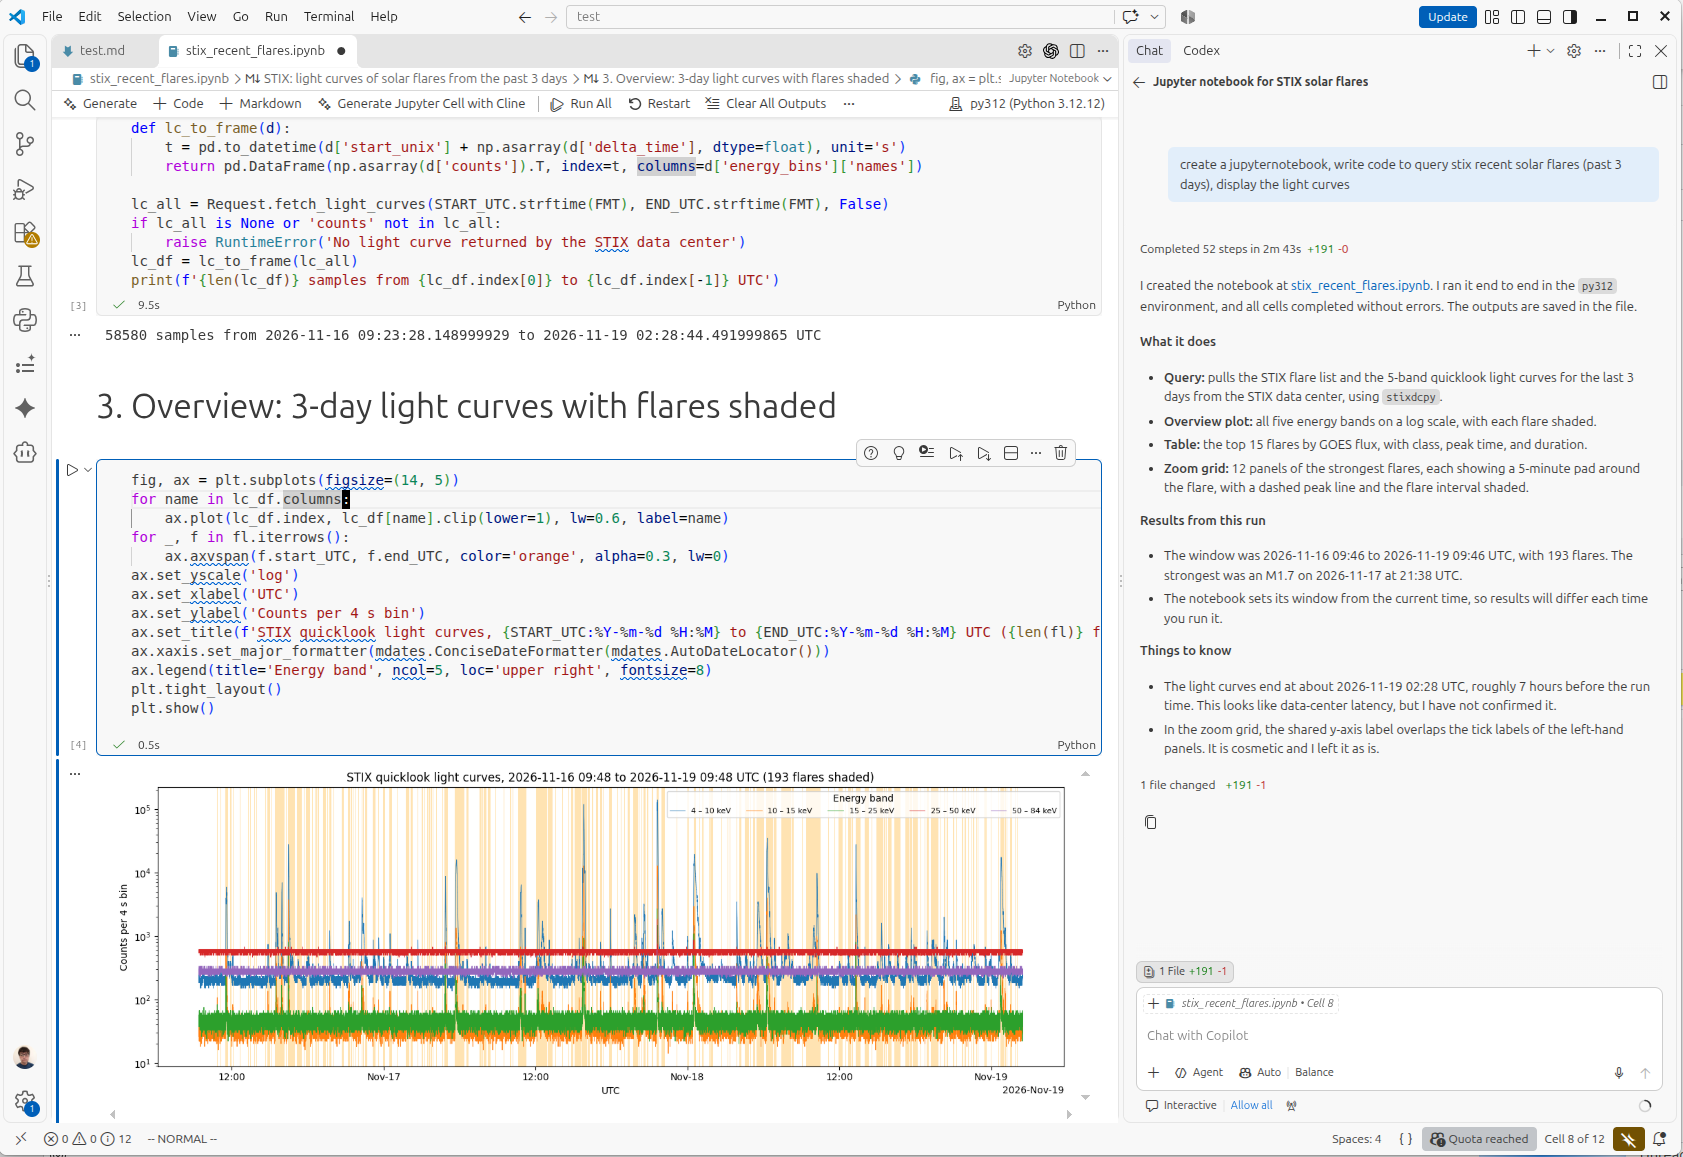
\includegraphics[width=\linewidth]{figures/pyexample.png}
    \caption{Python notebook example showing assistant-generated code and a STIX
      quicklook light-curve overview.}
    \label{fig:assistant-python}
  \end{subfigure}\hfill
  \begin{subfigure}[t]{0.49\linewidth}
    \centering
    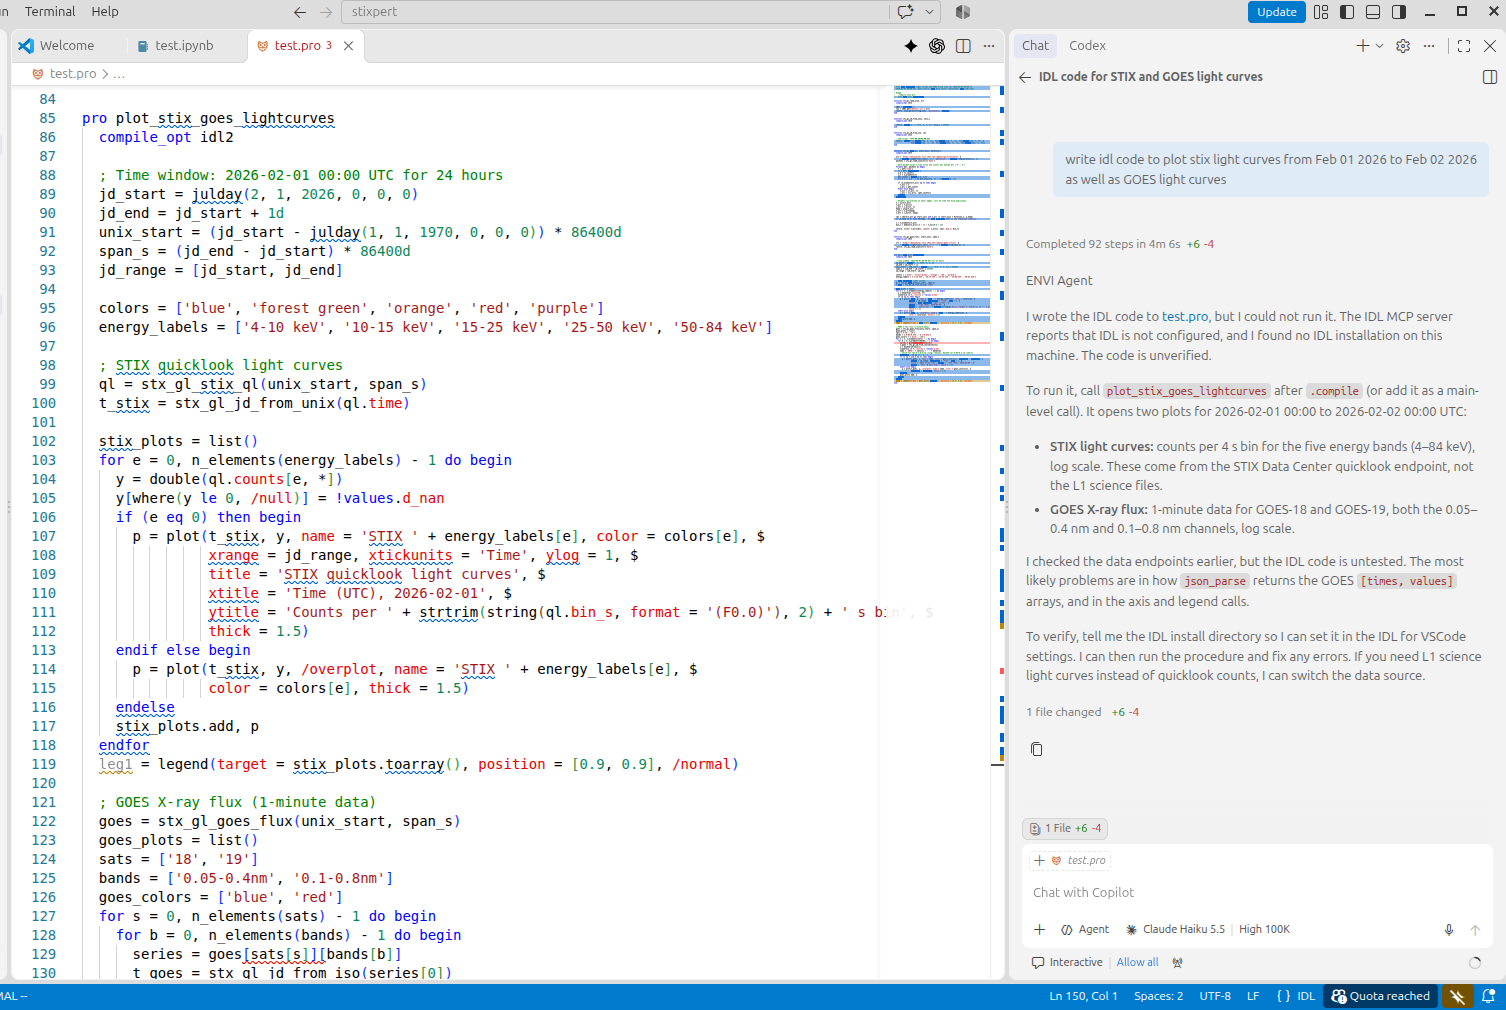
\includegraphics[width=\linewidth]{figures/idlexample.png}
    \caption{IDL example for plotting STIX and GOES light curves; the assistant
      reports that this code could not be run and remains unverified.}
    \label{fig:assistant-idl}
  \end{subfigure}
  \caption{Examples of solar-analysis code generated with AI assistance in Python and IDL.
    The screenshots illustrate code-generation workflows, not a controlled comparison of
    equivalent implementations: the Python panel shows a plotted result, whereas the IDL
    panel explicitly notes that its code was not executed.
  }
  \label{fig:assistant-code-examples}
\end{figure}

\section{Discussion and conclusions}
\label{sec:discussion}

StiXpert explores a way to lower the practical barrier between a solar-physics question
and the distributed knowledge needed to investigate it.
Its central value is to help researchers retrieve and connect information about
instruments, observations, data products, and analysis methods across a heterogeneous
solar-physics landscape.
Code assistance is one possible consequence of that discovery process, not the system's
sole purpose.
StiXpert is not intended to replace an instrument scientist or researcher, but to make
relevant expertise easier to find and apply.
Although developed around STIX, its indexed multi-instrument SSWIDL software and
broader flare and Solar Orbiter context support discovery and analysis workflows that
use STIX alongside complementary observations.
A curated knowledge base can help researchers discover candidate observations and
relevant methods, understand instrument products and processing algorithms, and find
the software resources needed to pursue an analysis.
The source-grounded design also creates a channel through which instrument teams can
make their software knowledge, examples, and carefully scoped analysis pipelines more
accessible.

The separation between indexed knowledge and client-side execution is important.
In the reference configuration, the MCP server searches its local index and can
statically validate Python scripts against indexed names and selected public endpoints;
it does not run analysis scripts or fetch the data itself.
The executed Python example therefore reflects client-side code and data access, while
the IDL example remains unexecuted because the required environment was unavailable.
Static indexing can become stale as packages evolve, and a passing code check cannot
establish scientific correctness.
Researchers must inspect provenance, test scripts against selected data, and retain
responsibility for calibration choices and physical conclusions.
The examples here demonstrate an interaction pattern, not a measured improvement in
research productivity or a general validation of AI-generated scientific analysis.

\subsection{Future perspectives}
\label{sec:future}

Future work should evaluate the system on a documented event set and report the accuracy
and completeness of retrieved knowledge, whether answers are supported by relevant
sources, the usefulness of observation and method discovery, code execution rates,
cross-language agreement, provenance completeness, and expert-rated scientific
reasoning quality.
A useful next step is to repeat both demonstrations in pinned Python and SSWIDL
environments, independently verify observation coverage, and compare time-aligned light
curves with stated tolerances.
Further extension of the indexed knowledge to additional instruments, data services,
and analysis environments could deepen coordinated analysis across observatories,
provided that time standards, calibration status, coordinate frames, and data
provenance are represented explicitly.

More capable agents may eventually help formulate follow-up questions, identify
under-explored combinations of observations, or suggest candidate research gaps.
Such suggestions should be treated as hypotheses for expert review, not as evidence
that a gap exists or a discovery has been made.
With transparent knowledge sources, controlled tools, reproducible workflows, and human
oversight, AI assistants may open a new mode of interaction with scientific data and
software while allowing researchers and instrument teams to focus more of their effort
on physical questions and instrument-specific science.


\bibliographystyle{elsarticle-num-names}
\bibliography{bibsample}

\end{document}
